% $Id: LogErr_desdoc.tex,v 1.10 2003/09/02 17:50:01 cdeluca Exp $
%
% Earth System Modeling Framework
% Copyright 2002-2003, University Corporation for Atmospheric Research,
% Massachusetts Institute of Technology, Geophysical Fluid Dynamics
% Laboratory, University of Michigan, National Centers for Environmental
% Prediction, Los Alamos National Laboratory, Argonne National Laboratory,
% NASA Goddard Space Flight Center.
% Licensed under the GPL.
\documentclass[]{article}
\usepackage{epsf}
\usepackage{html}
\usepackage{times}
\usepackage[T1]{fontenc}
\usepackage[dvips]{graphics,color}
\textwidth 6.5in
\textheight 8.5in
\addtolength{\oddsidemargin}{-.75in}
\newcommand{\mytitle}{LogErr design}
\newcommand{\myauthors}{Shep Smithline and Erik Kluzek}
\begin{document}
\bodytext{BGCOLOR=white LINK=#083194 VLINK=#21004A}
% Title page
% $Id: title_alldoc.tex,v 1.14 2012/01/06 20:15:12 svasquez Exp $
%
% Earth System Modeling Framework
% Copyright 2002-2013, University Corporation for Atmospheric Research, 
% Massachusetts Institute of Technology, Geophysical Fluid Dynamics 
% Laboratory, University of Michigan, National Centers for Environmental 
% Prediction, Los Alamos National Laboratory, Argonne National Laboratory, 
% NASA Goddard Space Flight Center.
% Licensed under the University of Illinois-NCSA License.


\begin{titlepage}

\begin{center}
{\Large Earth System Modeling Framework } \\
\vspace{.25in}
{\Large {\bf \mytitle}} \\
\vspace{.75in}
{\large {\it \myauthors}} \\
\vspace{.25in}
{\large {\today}}
\vspace{.25in}
\end{center}

\begin{latexonly}
\vspace{4.5in}
\begin{tabular}{p{5in}p{.9in}}
\hrulefill \\
\noindent {\bf NASA Earth Science Technology Office} \\
\noindent Computational Technologies Project \\
\noindent CAN 00-OES-01 \\
\noindent http://www.earthsystemmodeling.org \\
\end{tabular}
\end{latexonly}

\end{titlepage}















\newpage
\tableofcontents
\newpage
\section{Synopsis}
% $Id: LogErr_syn.tex,v 1.4 2006/11/16 05:21:08 cdeluca Exp $
%
% Earth System Modeling Framework
% Copyright 2002-2008, University Corporation for Atmospheric Research, 
% Massachusetts Institute of Technology, Geophysical Fluid Dynamics 
% Laboratory, University of Michigan, National Centers for Environmental 
% Prediction, Los Alamos National Laboratory, Argonne National Laboratory, 
% NASA Goddard Space Flight Center.
% Licensed under the University of Illinois-NCSA License.

%\section{Synopsis}

The {\tt ESMF\_Log} object provides an interface for user to print out log
information, as well as error and warning information.   This information may 
either go to standard out or to files.

%\section{Algorithmic Description}
%% $Id: LogErr_alg.tex,v 1.1 2003/03/28 21:33:06 shep_smith Exp $
%
% Earth System Modeling Framework
% Copyright 2002-2003, University Corporation for Atmospheric Research, 
% Massachusetts Institute of Technology, Geophysical Fluid Dynamics 
% Laboratory, University of Michigan, National Centers for Environmental 
% Prediction, Los Alamos National Laboratory, Argonne National Laboratory, 
% NASA Goddard Space Flight Center.
% Licensed under the GPL.

%\section{Algorithmic Description}

<Description of the continuous and discrete scientific algorithms used
in the software.  May reference rather than describe algorithms explicitly.>




\section{Object Model}
%$Id: LogErr_obj.tex,v 1.8 2010/03/04 18:57:44 svasquez Exp $
%
% Earth System Modeling Framework
% Copyright 2002-2010, University Corporation for Atmospheric Research, 
% Massachusetts Institute of Technology, Geophysical Fluid Dynamics 
% Laboratory, University of Michigan, National Centers for Environmental 
% Prediction, Los Alamos National Laboratory, Argonne National Laboratory, 
% NASA Goddard Space Flight Center.
% Licensed under the University of Illinois-NCSA License.

%\section{Object Model}

The following is a simplified UML diagram showing the structure of the
Log class.  See Appendix A, {\it A Brief Introduction to UML},
for a translation table that lists the symbols in the diagram and their 
meaning.

\begin{center}
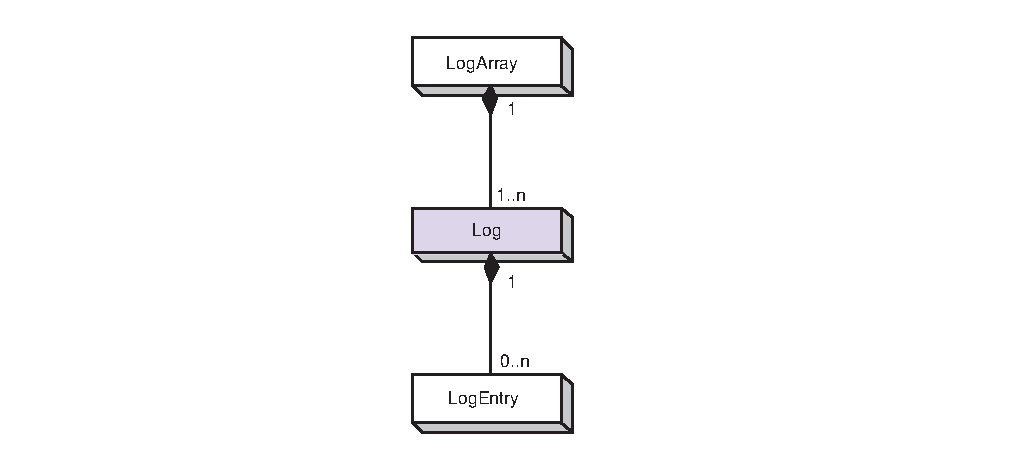
\includegraphics{Log_obj}   
\end{center}


\section{Global Parameters and Definitions}
%                **** IMPORTANT NOTICE *****
% This LaTeX file has been automatically produced by ProTeX v. 1.1
% Any changes made to this file will likely be lost next time
% this file is regenerated from its source. Send questions 
% to Arlindo da Silva, dasilva@gsfc.nasa.gov
 
\setlength{\parskip}{0pt}
\setlength{\parindent}{0pt}
\setlength{\baselineskip}{11pt}
 
%--------------------- SHORT-HAND MACROS ----------------------
\def\bv{\begin{verbatim}}
\def\ev{\end{verbatim}}
\def\be{\begin{equation}}
\def\ee{\end{equation}}
\def\bea{\begin{eqnarray}}
\def\eea{\end{eqnarray}}
\def\bi{\begin{itemize}}
\def\ei{\end{itemize}}
\def\bn{\begin{enumerate}}
\def\en{\end{enumerate}}
\def\bd{\begin{description}}
\def\ed{\end{description}}
\def\({\left (}
\def\){\right )}
\def\[{\left [}
\def\]{\right ]}
\def\<{\left  \langle}
\def\>{\right \rangle}
\def\cI{{\cal I}}
\def\diag{\mathop{\rm diag}}
\def\tr{\mathop{\rm tr}}
%-------------------------------------------------------------

\markboth{Left}{Source File: ESMF\_LogConstants.inc,  Date: Fri Mar 28 16:24:52 EST 2003
}

 
%/////////////////////////////////////////////////////////////

 ESMF\_SINGLE\_FILE: write log output to a single file 
%/////////////////////////////////////////////////////////////
 
\mbox{}\hrulefill\ 
 

 ESMF\_MULT\_LOG\_FILE: write log output to multiple files 
%/////////////////////////////////////////////////////////////
 
\mbox{}\hrulefill\ 
 

 ESMF\_LOG\_TRUE: integer to signify true statement 
%/////////////////////////////////////////////////////////////
 
\mbox{}\hrulefill\ 
 

 ESMF\_LOG\_FALSE: integer to signify false statement 
%/////////////////////////////////////////////////////////////
 
\mbox{}\hrulefill\ 
 

 ESMF\_LOG\_UNIT\_NUMBER: used to create fortran unit numbers 
%/////////////////////////////////////////////////////////////
 
\mbox{}\hrulefill\ 
 

 ESMF\_LOG\_FORT\_STDOUT: standard out for Fortran 
%/////////////////////////////////////////////////////////////
 
\mbox{}\hrulefill\ 
 

 ESMF\_LOG\_UPPER: upper bound for fortran unit number
%...............................................................

%                **** IMPORTANT NOTICE *****
% This LaTeX file has been automatically produced by ProTeX v. 1.1
% Any changes made to this file will likely be lost next time
% this file is regenerated from its source. Send questions 
% to Arlindo da Silva, dasilva@gsfc.nasa.gov
 
\setlength{\parskip}{0pt}
\setlength{\parindent}{0pt}
\setlength{\baselineskip}{11pt}
 
%--------------------- SHORT-HAND MACROS ----------------------
\def\bv{\begin{verbatim}}
\def\ev{\end{verbatim}}
\def\be{\begin{equation}}
\def\ee{\end{equation}}
\def\bea{\begin{eqnarray}}
\def\eea{\end{eqnarray}}
\def\bi{\begin{itemize}}
\def\ei{\end{itemize}}
\def\bn{\begin{enumerate}}
\def\en{\end{enumerate}}
\def\bd{\begin{description}}
\def\ed{\end{description}}
\def\({\left (}
\def\){\right )}
\def\[{\left [}
\def\]{\right ]}
\def\<{\left  \langle}
\def\>{\right \rangle}
\def\cI{{\cal I}}
\def\diag{\mathop{\rm diag}}
\def\tr{\mathop{\rm tr}}
%-------------------------------------------------------------

\markboth{Left}{Source File: ESMF\_ErrConstants.inc,  Date: Fri Mar 28 16:27:02 EST 2003
}

 
%/////////////////////////////////////////////////////////////

  ESMF\_FATAL : Fatal error 
%/////////////////////////////////////////////////////////////
 
\mbox{}\hrulefill\ 
 

  ESMF\_WARNING : Non-Fatal error 
%/////////////////////////////////////////////////////////////
 
\mbox{}\hrulefill\ 
 

  ESMF\_SINGLE\_ERR\_FILE : Send errors to single file for all PE's 
%/////////////////////////////////////////////////////////////
 
\mbox{}\hrulefill\ 
 

  ESMF\_MULT\_ERR\_FILE : All PE's write to seperate files. 
%/////////////////////////////////////////////////////////////
 
\mbox{}\hrulefill\ 
 

  ESMF\_ERR\_RETURN : Return on error 
%/////////////////////////////////////////////////////////////
 
\mbox{}\hrulefill\ 
 

  ESMF\_ERR\_REPORT : Print a detailed error report. 
%/////////////////////////////////////////////////////////////
 
\mbox{}\hrulefill\ 
 

  ESMF\_WARNINGS\_FATAL : Execution will terminate on warnings. 
%/////////////////////////////////////////////////////////////
 
\mbox{}\hrulefill\ 
 

  ESMF\_WARNINGS\_NOT\_FATAL : Execution will not terminate on warnings 
%/////////////////////////////////////////////////////////////
 
\mbox{}\hrulefill\ 
 

   These are the generic error codes.  The user is free to add
   additional messages within the source code. 
%/////////////////////////////////////////////////////////////
 
\mbox{}\hrulefill\ 
 

  ESMF\_ERR\_MEM : Unable to allocate requested memory 
%/////////////////////////////////////////////////////////////
 
\mbox{}\hrulefill\ 
 

  ESMF\_ERR\_SUP : No support for requested operation 
%/////////////////////////////////////////////////////////////
 
\mbox{}\hrulefill\ 
 

  ESMF\_ERR\_SIG : Signal received 
%/////////////////////////////////////////////////////////////
 
\mbox{}\hrulefill\ 
 

  ESMF\_ERR\_FP : Floating point exception 
%/////////////////////////////////////////////////////////////
 
\mbox{}\hrulefill\ 
 

  ESMF\_ERR\_COR : Corrupted ESMF object detected 
%/////////////////////////////////////////////////////////////
 
\mbox{}\hrulefill\ 
 

  ESMF\_ERR\_LIB : Error in library called by ESMF 
%/////////////////////////////////////////////////////////////
 
\mbox{}\hrulefill\ 
 

  ESMF\_ERR\_PLIB : ESMF generated inconsistent data 
%/////////////////////////////////////////////////////////////
 
\mbox{}\hrulefill\ 
 

  ESMF\_ERR\_MEMC : Memory corrupted 
%/////////////////////////////////////////////////////////////
 
\mbox{}\hrulefill\ 
 

  ESMF\_ERR\_BUSY : Resource is busy 
%/////////////////////////////////////////////////////////////
 
\mbox{}\hrulefill\ 
 

  ESMF\_ERR\_SYS : System call error 
%/////////////////////////////////////////////////////////////
 
\mbox{}\hrulefill\ 
 

  ESMF\_ERR\_ARG\_SIZ : Non-comforming object sizes used in operation 
%/////////////////////////////////////////////////////////////
 
\mbox{}\hrulefill\ 
 

  ESMF\_ERR\_ARG\_IDN : Two arguments not allowed to be the same 
%/////////////////////////////////////////////////////////////
 
\mbox{}\hrulefill\ 
 

  ESMF\_ERR\_ARG\_WRONG : Wrong argument 
%/////////////////////////////////////////////////////////////
 
\mbox{}\hrulefill\ 
 

  ESMF\_ERR\_ARG\_CORRUPT : Null or corrupeted ESMF object sent in as argument 
%/////////////////////////////////////////////////////////////
 
\mbox{}\hrulefill\ 
 

  ESMF\_ERR\_ARG\_OUTOFRANGE : Input argument out of range 
%/////////////////////////////////////////////////////////////
 
\mbox{}\hrulefill\ 
 

  ESMF\_ERR\_ARG\_BADPTR : Invalid pointer argument 
%/////////////////////////////////////////////////////////////
 
\mbox{}\hrulefill\ 
 

  ESMF\_ERR\_ARG\_NOTSAMETYPE : Two arguments must be same object type 
%/////////////////////////////////////////////////////////////
 
\mbox{}\hrulefill\ 
 

  ESMF\_ERR\_ARG\_NOTSAMECOMM : Two arguments must have the same communicators 
%/////////////////////////////////////////////////////////////
 
\mbox{}\hrulefill\ 
 

  ESMF\_ERR\_ARG\_WRONGSTATE : Object in argument is in wrong state 
%/////////////////////////////////////////////////////////////
 
\mbox{}\hrulefill\ 
 

  ESMF\_ERR\_ARG\_INCOMP : Arguments are incompatible 
%/////////////////////////////////////////////////////////////
 
\mbox{}\hrulefill\ 
 

  ESMF\_ERR\_FILE\_OPEN : Unable to open file 
%/////////////////////////////////////////////////////////////
 
\mbox{}\hrulefill\ 
 

  ESMF\_ERR\_FILE\_READ : Unable to read from file 
%/////////////////////////////////////////////////////////////
 
\mbox{}\hrulefill\ 
 

  ESMF\_ERR\_FILE\_WRITE : Unable to write to file 
%/////////////////////////////////////////////////////////////
 
\mbox{}\hrulefill\ 
 

  ESMF\_ERR\_FILE\_UNEXPECTED : Unexpected data in file 
%/////////////////////////////////////////////////////////////
 
\mbox{}\hrulefill\ 
 

  ESMF\_ERR\_FILE\_CLOSE : Unable to close file 
%/////////////////////////////////////////////////////////////
 
\mbox{}\hrulefill\ 
 

  ESMF\_ERR\_INIT : Init method not called 
%/////////////////////////////////////////////////////////////
 
\mbox{}\hrulefill\ 
 

  ESMF\_ERR\_FILE\_ACTIVE : Instrumented region  is still active
%...............................................................

\section{LogErr Design}
\subsection{Description}
% $Id: LogErr_desc.tex,v 1.4 2004/03/16 20:04:11 cdeluca Exp $
%
% Earth System Modeling Framework
% Copyright 2002-2003, University Corporation for Atmospheric Research, 
% Massachusetts Institute of Technology, Geophysical Fluid Dynamics 
% Laboratory, University of Michigan, National Centers for Environmental 
% Prediction, Los Alamos National Laboratory, Argonne National Laboratory, 
% NASA Goddard Space Flight Center.
% Licensed under the GPL.

%\subsection{Description}

The Log class consists of a variety of methods for writing error, warning, 
and other messages to files or to standard out.  Options include the ability 
to write to a single file or multiple files, to write from a root PE or 
from all active PEs, and to halt at errors, at warnings, or never.  The 
verbosity of ouput can be adjusted with a flag.  Multiple 
Logs can be created within an application.  Logs may be given
user-specified names, or, if desired, a default {\tt ESMF\_Log\_World} can 
be used.  

Log provides capabilities to write to a file immediately or store entries 
in a buffer for writing either when the buffer is full, or when the user
calls an {\tt ESMF_LogFlush()} command.  The user can specify the number 
of entries that a Log should contain when it is flushed.  For buffered output, 
it's also possible to specify whether Log entries should be ordered or not.  


\subsection{Design}
% $Id: LogErr_design.tex,v 1.1 2003/03/28 21:33:08 shep_smith Exp $
%
% Earth System Modeling Framework
% Copyright 2002-2003, University Corporation for Atmospheric Research, 
% Massachusetts Institute of Technology, Geophysical Fluid Dynamics 
% Laboratory, University of Michigan, National Centers for Environmental 
% Prediction, Los Alamos National Laboratory, Argonne National Laboratory, 
% NASA Goddard Space Flight Center.
% Licensed under the GPL.

%\subsection{Design/Implementation}

There are two aspects to the design of the Log class.  The first is the actual class
itself, and the second is Fortran interface to the Log class. The design of
the Log class is pretty straightforward. 
Although the class contains a large number of methods, the most important methods
are ESMF\_LogInit, for initializing data; ESMF\_LogOpenFile and ESMF\_CloseFile,
for opening and closing output files; and ESMF\_LogInfo, ESMF\_LogErr, and ESMF\_LWarn, for
writing miscellaneous information, error, and warning information. In addition, there are
a variety of other methods that allow the user to control other behavior such whether
or not to stop execution on encountering errors or warnings, whether output
should be flushed from buffers to files automatically, or whether output should be verbose
or not.

The Log class was implemented in C/C++, but uses the Fortran I/O libraries when
the class methods are called from the Fortran wrappers. We forced the C/C++ methods 
to use the Fortran I/O library by creating 
utility functions, written in Fortran, but callable from Log's C++ methods,
which call the standard Fortran write, open and close functions.  We chose this 
approach because we still wanted to allow users to write to the Log files using the
standard Fortran write statements if they chose to.
Since you could conceivably be writing to the same file using 
both ESMF\_LogInfo, for example,  and the standard Fortran  write(),
both approaches have to use the same I/O 
libraries to avoid any collisions.  Since we can't force the Fortran write() to use the
C I/O libraries, our only alternative was to force our routines to use Fortran I/O
libraries.  Note: if you call the Log methods from C/C++ code, you bypass the wrappers
and all I/O is done with the C I/O libraries.

The design of the Fortran interface is relatively straightforward, but there are some
inter-language operability issues here as well.
Because the ESMF\_LogInfo routine needed to
take a variable number of arguments, the Fortran wrapper needed to be implemented in C.
To keep things as uniform as possible, all of the other wrapper functions were implemented
in C as well, except for ESMF\_LogInit(). We wanted to overload this function, and since
you can't overload functions in C, we needed to implement the code in another language.
Fortran was the obvious choice.





\subsubsection{Class Definition}
% $Id: LogErr_def.tex,v 1.1 2003/03/28 21:33:07 shep_smith Exp $
%
% Earth System Modeling Framework
% Copyright 2002-2003, University Corporation for Atmospheric Research, 
% Massachusetts Institute of Technology, Geophysical Fluid Dynamics 
% Laboratory, University of Michigan, National Centers for Environmental 
% Prediction, Los Alamos National Laboratory, Argonne National Laboratory, 
% NASA Goddard Space Flight Center.
% Licensed under the GPL.

%\subsubsection{Class Definition}

<Show internal attributes and methods of derived type, structure or class.

 This definition can be expressed using a general language like UML 
 (see, e.g. ``The Unified Modeling Language Reference Manual,'' 
 Rumbaugh et. al. 1999) or using constructs from a specific language like 
 Fortran.>

\subsubsection{Restrictions}
% $Id: LogErr_rest.tex,v 1.19 2008/04/05 03:38:41 cdeluca Exp $
%
% Earth System Modeling Framework
% Copyright 2002-2008, University Corporation for Atmospheric Research, 
% Massachusetts Institute of Technology, Geophysical Fluid Dynamics 
% Laboratory, University of Michigan, National Centers for Environmental 
% Prediction, Los Alamos National Laboratory, Argonne National Laboratory, 
% NASA Goddard Space Flight Center.
% Licensed under the University of Illinois-NCSA License.

\begin{enumerate}

\item {\bf Line, file and method are only available when using the C 
preprocessor}
Message writing methods are expanded using the ESMF macro ESMF\_CONTEXT 
that adds the predefined symbolic constants \_\_LINE\_\_ and \_\_FILE\_\_ (or 
the ESMF constant ESMF\_FILENAME if defined) and the ESMF constant ESMF\_METHOD 
to the argument list.  Using these constants, we can associate a file name, 
line number and method name with the message.  If the CPP preprocessor is not 
used, this expansion will not be done and hence the ESMF macro ESMF\_CONTEXT 
can not be used, leaving the file name, line number and method out of the Log 
text.

\item{\bf Get and set methods are partially implemented.}
Currently, the {\tt ESMF\_LogGet()} and {\tt ESMF\_LogSet()} methods are 
partially implemented.   

\item{\bf Log only appends entries.}
All writing to the Log is appended rather than overwriting the Log.  Future 
enhancements include the option to either append to an existing Log or 
overwrite the existing Log.

\item{\bf Avoiding conflicts with the default Log.}
The private methods {\tt ESMF\_LogInitialize()} and {\tt ESMF\_LogFinalize()} 
are called during {\tt ESMF\_Initialize()} and {\tt ESMF\_Finalize()} 
respectively, so they do not need to be called if the default Log is used. 
If a new Log is required, {\tt ESMF\_LogOpen()} is used with a new Log object 
passed in so that there are no conflicts with the default Log.

\item{\bf ESMF\_LOG\_SINGLE does not work properly.}
When the {\tt ESMF\_LogType} is set to {\tt ESMF\_LOG\_SINGLE}, different system may behave
differently.  The log messages from some processors may be lost or overwritten
by other processors.  Users are advised not to use this mode.  The MPI-based
I/O will be implemented to fix the problem in the future release. 


\end{enumerate}

\section{LogErr F90 Interface}
\subsection{Use and Examples}
% $Id: LogErr_fex.tex,v 1.2 2003/08/07 17:54:18 shep_smith Exp $
%
% Earth System Modeling Framework
% Copyright 2002-2003, University Corporation for Atmospheric Research, 
% Massachusetts Institute of Technology, Geophysical Fluid Dynamics 
% Laboratory, University of Michigan, National Centers for Environmental 
% Prediction, Los Alamos National Laboratory, Argonne National Laboratory, 
% NASA Goddard Space Flight Center.
% Licensed under the GPL.

%\subsection{F90 Use and Examples}

%<Detailed examples of F90 usage of the class.>


\subsubsection{Example 1. Simple Example.}

In this example we use the default ESMF\_Log\_World object and illustrate
the ESMF\_LogGetUnit()to write to
the log file aLog.txt.

{\tt
\begin{verbatim}
program test_log
  use ESMF_Mod
  implicit none
#include "ESMC_LogErr.inc"
  call ESMF_LogOpenFile(ESMF_Log_World,ESMF_SINGLE_LOG_FILE,"aLog.txt")
  write(ESMF_LogGetUnit(ESMF_Log_World),*)"This is a test."
  call ESMF_LogCloseFile(ESMF_Log_World)
end program
\end{verbatim}
\tt}

\subsubsection{Example 2. Simple Error Handling.}

Here we illustrate simple error handling.  We define an error handler - anErr -
and error output goes to the
file anErr.txt.  There are four options that can be set with ESMF\_LogSet()
and we set them all here: verbose (whether an
error message should be written for anErr), flush (whether output should be 
flushed), haltOnErr and haltOnWarn (whether the code should halt on
an error or warning).  While the values set here are the default
values, so they need not be set with ESMF\_Set(), the example illustrates how
to ESMF\_SET().

{\tt
\begin{verbatim}
#include "ESMC_LogErr.inc" 
type(ESMF_Log) :: anErr
integer returnCode 
call ESMF_LogSet(anErr, verbose=ESMF_TF_TRUE, flush=ESMF_TF_FALSE,   &
                 haltOnErr=ESMF_TF_TRUE, haltOnWarn=ESMF_TF_FALSE)
call ESMF_LogOpenFile(anErr,ESMF_SINGLE_LOG_FILE,"anErr.txt")
returnCode=foo()
if (returnCode == ESMF_FATAL) call ESMF_LogErr(anErr, returnCode) 
call ESMF_LogCloseFile(anErr)
\end{verbatim}
\tt}

\subsubsection{Example 3. More error handling.}

In this example, we illustrate more complex error handling.  We use
ESMF\_LogGet() to get the value of verbose and if it's set to ESMF\_TF\_TRUE
then turn off verbose midway through the code.  This allows you to put in lots
of debugging code, and then if you want to turn them off, you can just call
an ESMF\_LogSet() rather than commenting out all the error handling calls.
We also illustrate the use 
of ESMF\_LogErrMsg() which writes an additional message to the err file.

{\tt
\begin{verbatim}
#include "ESMC_LogErr.inc" 
type(ESMF_Log) :: anErr
type(ESMF_Logical) :: myVerbosity
character(len=32) :: myMsg
integer returnCode 
call ESMF_LogSet(anErr, verbose=ESMF_TF_TRUE, flush=ESMF_TF_FALSE,   &
                 haltOnErr=ESMF_TF_TRUE, haltOnWarn=ESMF_TF_FALSE)
call ESMF_LogOpenFile(anErr,ESMF_SINGLE_LOG_FILE,"anErr.txt")
returnCode=foo()
myMsg="This will be written out."
if (returnCode == ESMF_FATAL) call ESMF_LogErrMsg(anErr, returnCode,myMsg) 
ESMF_LogGet(anErr,verbose=myVerbosity)
if (myVerbosity==ESMF_TF_TRUE) call ESMF_LogSet(verbose=ESMF_TF_FALSE)
myMsg="This will not be written out."
returnCode=foo()
if (returnCode == ESMF_FATAL) call ESMF_LogErrMsg(anErr, returnCode,myMsg)
call ESMF_LogCloseFile(anErr)
\end{verbatim}
\tt}





%#\subsection{Parameters}
%#% $Id: class_fparam.tex,v 1.5 2007/03/31 05:50:45 cdeluca Exp $
%
% Earth System Modeling Framework
% Copyright 2002-2007, University Corporation for Atmospheric Research, 
% Massachusetts Institute of Technology, Geophysical Fluid Dynamics 
% Laboratory, University of Michigan, National Centers for Environmental 
% Prediction, Los Alamos National Laboratory, Argonne National Laboratory, 
% NASA Goddard Space Flight Center.
% Licensed under the University of Illinois-NCSA License.

%\subsection{Parameters}

\begin{description}

\item [<ITEM1>] <Description of ITEM1.>

\item [<ITEM2>] <Description of ITEM2.>

\end{description}









%\subsection{Class API}
%                **** IMPORTANT NOTICE *****
% This LaTeX file has been automatically produced by ProTeX v. 1.1
% Any changes made to this file will likely be lost next time
% this file is regenerated from its source. Send questions 
% to Arlindo da Silva, dasilva@gsfc.nasa.gov
 
\setlength{\parskip}{0pt}
\setlength{\parindent}{0pt}
\setlength{\baselineskip}{11pt}
 
%--------------------- SHORT-HAND MACROS ----------------------
\def\bv{\begin{verbatim}}
\def\ev{\end{verbatim}}
\def\be{\begin{equation}}
\def\ee{\end{equation}}
\def\bea{\begin{eqnarray}}
\def\eea{\end{eqnarray}}
\def\bi{\begin{itemize}}
\def\ei{\end{itemize}}
\def\bn{\begin{enumerate}}
\def\en{\end{enumerate}}
\def\bd{\begin{description}}
\def\ed{\end{description}}
\def\({\left (}
\def\){\right )}
\def\[{\left [}
\def\]{\right ]}
\def\<{\left  \langle}
\def\>{\right \rangle}
\def\cI{{\cal I}}
\def\diag{\mathop{\rm diag}}
\def\tr{\mathop{\rm tr}}
%-------------------------------------------------------------

\markboth{Left}{Source File: ESMF\_LogErr.F90,  Date: Thu Mar 27 16:05:15 EST 2003
}

 
%/////////////////////////////////////////////////////////////

  ============================================================================\subsection{Fortran:  Module Interface Fortran Interface to Log class.  (Source File: ESMF\_LogErr.F90)}


  
  
   The Fortran interface to the Log class is written in both Fortran and C/C++.
   This file contains the interface code written in Fortran.  It also contains
   some utility functions used by the Log class.
  
  ============================================================================
  
\bigskip{\sf PRIVATE TYPES:}
\begin{verbatim} private
 type:: ESMF_Log
     sequence
     integer oneLogErrFile     !An ESMF_Log object will write to one file if
 			      !oneLogErrFile is set to ESMF_LOG_TRUE.
 
     integer standardOut       !An ESMF_Log object will write to the screen if
 			      !standardOut is set to ESMF_LOG_TRUE.
 
     integer fortIsOpen        !If fortIsOpen is set to ESMF_LOG_TRUE, an 
 			      !ESMF_Log object has a fortran file open.
 
     integer unitNumber        !Fortran unit number for output
 
     integer numFilePtr        !Index into global array of Fortran unit numbers 
 
     integer verboseSet        !An ESMF_Log object will write output only if
 			      !verbose is set to ESMF_LOG_TRUE.
     
     integer flushSet          !An ESMF_Log object will have its output flushed
 			      !if flushSet is set to ESMF_LOG_TRUE.
 
     integer haltOnWarn        !An ESMF_Log object will halt on encountering
 			      !a warning if haltOnWarn is set to ESMF_LOG_TRUE. 
 
     integer haltOnErr         !An ESMF_Log object will halt on encountering
 			      !an error if haltOnErr is set to ESMF_LOG_TRUE. 
 
     character(len=32) nameLogErrFile !Name of an ESMF_Log objects's output file 
 
 end type ESMF_Log\end{verbatim}
 
%/////////////////////////////////////////////////////////////
 
\mbox{}\hrulefill\ 
 

   !PUBLIC MEMBER Functions\subsubsection [ESMF\_LogInit] {ESMF\_LogInit - initialize an error object.}


  
\bigskip{\sf INTERFACE:}
\begin{verbatim} subroutine ESMF_LogInit(aLog,verbose, flush,standardOut,haltOnErr,haltOnWarn)\end{verbatim}{\em ARGUMENTS:}
\begin{verbatim}  type(ESMF_Log), intent(in) :: aLog
  integer, intent(inout),optional::verbose, flush, standardOut,haltOnErr,haltOnWarn \end{verbatim}
{\sf DESCRIPTION:\\ }


     Most of the Fortran wrapper routines for the C/C++ ESMC\_Log class are
     written in C. This is the only routine that isn't. See the class design
     section for the rational for doing this. 
  
     With the exception of the ESMF\_Log object, all the arguments are optional.
     See the Examples section of the document for a discussion of how to use the
     routine.
   
%/////////////////////////////////////////////////////////////
 
\mbox{}\hrulefill\ 
 
\subsubsection [ESMF\_LogCloseFortran] {ESMF\_LogCloseFortran}


  
\bigskip{\sf INTERFACE:}
\begin{verbatim} subroutine ESMF_LogCloseFortran(unitNumber)\end{verbatim}{\em ARGUMENTS:}
\begin{verbatim}     integer, intent(in) :: unitNumber\end{verbatim}
{\sf DESCRIPTION:\\ }


   This routine closes any log files that have been written to using
   the Fortran interface.  It is called by by the C/C++ Log
   method ESMC\_LogFinalize().
   Note: This routine is not a module procedure
   because it needs to be called from Log's C++ method and
   F90 mangles the names of functions
   inside modules.
   
%/////////////////////////////////////////////////////////////
 
\mbox{}\hrulefill\ 
 
\subsubsection [ESMF\_LogOpenFortran] {ESMF\_LogOpenFortran}


  
\bigskip{\sf INTERFACE:}
\begin{verbatim} subroutine ESMF_LogOpenFortran(isOpen,unitNumber, nameLogFile)
   implicit none\end{verbatim}{\em ARGUMENTS:}
\begin{verbatim}   integer, intent(inout) ::  unitNumber !standard Fortran unit number for I/O
 
   integer, intent(inout) ::  isOpen     !if file successfully opened
 				        !isOpen set to ESMF_LOG_TRUE	
 					!otherwise set to ESMF_LOG_FALSE
 
   character (len=32), intent(in) :: nameLogFile
      \end{verbatim}
{\sf DESCRIPTION:\\ }


   This routine opens the log file and is called by ESMC\_LogWrite.
   See the ESMC\_LogErr.C file for more details.
   This routine is not a module procedure because F90 mangles
   the names of functions
   inside modules and this routine is called by ESMC\_LogWrite() - a C++
   method.
   
%/////////////////////////////////////////////////////////////
 
\mbox{}\hrulefill\ 
 
\subsubsection [ESMF\_LogPrintChar] {ESMF\_LogPrintChar - Prints a character and an optional }


                                   message
  
\bigskip{\sf INTERFACE:}
\begin{verbatim}  subroutine ESMF_LogPrintChar(unitNumber,charData,flushSet,msg,length)\end{verbatim}
 
%/////////////////////////////////////////////////////////////
 
\mbox{}\hrulefill\ 
 

\bigskip{\em ARGUMENTS:}
\begin{verbatim}   integer, intent(in)::unitNumber,flushSet !See ESMF_Log data type
 
   character, intent(in)::charData          !character to be printed out
 
   character(len=32), intent(in):: msg      !optional message; only
 					   !printed out if length is
 					   !greater than zero.\end{verbatim}
{\sf DESCRIPTION:\\ }


   This routine, and the routines that follow it, are used by ESMC\_LogPrint()
   ESMC\_LogPrintHeader() in the Log class.  Ordinarily, these Log routines would
   have just used fprintf.  However, because we needed to use the Fortran I/O 
   libraries when calling Log from a Fortran code
   (see the discussion about the class design), we had to make 
   calls to ESMF\_LogPrintChar() and the subroutines below, in addition to
   C's fprintf() (We still have to support C/C++, so we still need fprintf() ).
   ESMF\_LogPrintChar() and the routines below are not particularly general,
   but do the trick. 
%/////////////////////////////////////////////////////////////
 
\mbox{}\hrulefill\ 
 

   \subsubsection [ESMF\_LogPrintNewLine] {ESMF\_LogPrintNewLine - prints a newline character}


  
\bigskip{\sf INTERFACE:}
\begin{verbatim}  subroutine ESMF_LogPrintNewLine(unitNumber,flushSet)\end{verbatim}
 
%/////////////////////////////////////////////////////////////
 
\mbox{}\hrulefill\ 
 

\bigskip{\em ARGUMENTS:}
\begin{verbatim}   integer, intent(in)::unitNumber,flushSet  !see above\end{verbatim}
{\sf DESCRIPTION:\\ }


   Prints a newline character.  See ESMF\_LogPrintChar for more 
   discussion 
%/////////////////////////////////////////////////////////////
 
\mbox{}\hrulefill\ 
 

  \subsubsection [ESMF\_LogPrintString] {ESMF\_LogPrintString - prints a string}


  
\bigskip{\sf INTERFACE:}
\begin{verbatim}  subroutine ESMF_LogPrintString(unitNumber,stringData,len1,flushSet,msg,len2)\end{verbatim}
 
%/////////////////////////////////////////////////////////////
 
\mbox{}\hrulefill\ 
 

\bigskip{\em ARGUMENTS:}
\begin{verbatim}   integer, intent(in)::unitNumber,flushSet,len1,len2
   character(len=32), intent(in)::msg,stringData\end{verbatim}
{\sf DESCRIPTION:\\ }


   Prints a string; see ESMF\_LogPrintChar() for a fuller discussion 
%/////////////////////////////////////////////////////////////
 
\mbox{}\hrulefill\ 
 
\subsubsection [ESMF\_LogPrintInt] {ESMF\_LogPrintInt - prints an int}


  
\bigskip{\sf INTERFACE:}
\begin{verbatim}  subroutine ESMF_LogPrintInt(unitnumber,intData,flushSet,msg,length)\end{verbatim}
 
%/////////////////////////////////////////////////////////////
 
\mbox{}\hrulefill\ 
 

\bigskip{\em ARGUMENTS:}
\begin{verbatim}   integer, intent(in)::unitNumber,flushSet,intData
   character(len=32), intent(in):: msg
   !DESCRIPTION
   Prints an integer; see ESMF\_LogPrintChar() for more details\end{verbatim}
 
%/////////////////////////////////////////////////////////////
 
\mbox{}\hrulefill\ 
 

\bigskip{\em ARGUMENTS:}
\begin{verbatim}   integer, intent(in)::unitNumber,flushSet
   real, intent(in):: floatData
   character(len=32), intent(in):: msg\end{verbatim}
{\sf DESCRIPTION:\\ }


   Prints a real number; see ESMF\_LogPrintChar() for a longer discussion
  
%...............................................................

\section{LogErr C++ Interface}
\subsection{Use and Examples}
% $Id$
%
% Earth System Modeling Framework
% Copyright (c) 2002-2024, University Corporation for Atmospheric Research, 
% Massachusetts Institute of Technology, Geophysical Fluid Dynamics 
% Laboratory, University of Michigan, National Centers for Environmental 
% Prediction, Los Alamos National Laboratory, Argonne National Laboratory, 
% NASA Goddard Space Flight Center.
% Licensed under the University of Illinois-NCSA License.

%\subsection{C++ Use and Examples}

%<Detailed examples of F90 usage of the class.>
\subsubsection{Example Code}

In this example we set the default log file to log.txt and then call the 
various methods to write to the log.  The first step is to include 
ESMC\_LogErr.h and ESMF\_LogMacros.inc.  Next, we define ESMC\_Method to 
the corresponding method.

{\tt
\begin{verbatim}
#include "ESMCI_LogErr.h"
#define ESMC_METHOD "TestLog1Ex"

int main() {
int *rc;
    
    ESMC_LogSetFilename("log1.txt");
    ESMC_LogDefault.WriteLog("LogWrite",ESMC_LOGMSG_WARN);
    ESMC_LogDefault.FoundError(ESMF_TRUE,rc);
	ESMC_LogDefault.MsgFoundError(ESMF_TRUE,"Log Msg Found Error",rc);
    ESMC_LogDefault.AllocError(rc);
	ESMC_LogDefault.MsgAllocError("Log Msg Alloc Error",rc);
}
\end{verbatim}
\tt}

\subsubsection{Example 1. ESMC\_LogSetFilename}

The default log is already set by ESMF during initialization.  However, if a user
wants to write to a different log, then ESMC\_LogSetFilename is used.  A fully 
qualified path and filename are required.  If only the filename is given then
the log file will be created in the same directory as the method calling the
ESMC\_LogSetFilename.

\subsubsection{Example 2. ESMC\_LogWrite}

ESMC\_LogWrite is the basic method for writing to the log.  All it requires is a
message and log type.

\subsubsection{Example 3. ESMC\_LogFoundError}

ESMC\_LogFoundError allows the user to pass a return code to check and if the 
return code is associated with an error it will write the corresponding error
message to the log.  It will also pass back the return code in rc.

\subsubsection{Example 4. ESMC\_LogMsgFoundError}

ESMC\_LogMsgFoundError does the same as ESMC\_LogFoundError but allows the user
to add his/her own message as well.

\subsubsection{Example 5. ESMC\_LogAllocError}

ESMC\_LogAllocError writes an allocation error to the log and returns a return
code rc.

\subsubsection{Example 6. ESMC\_LogMsgAllocError}

ESMC\_LogMsgAllocError does the same as ESMC\_LogAllocError but allows the user
to add his/her own message as well.

\subsection{Parameters}
%                **** IMPORTANT NOTICE *****
% This LaTeX file has been automatically produced by ProTeX v. 1.1
% Any changes made to this file will likely be lost next time
% this file is regenerated from its source. Send questions 
% to Arlindo da Silva, dasilva@gsfc.nasa.gov
 
\setlength{\parskip}{0pt}
\setlength{\parindent}{0pt}
\setlength{\baselineskip}{11pt}
 
%--------------------- SHORT-HAND MACROS ----------------------
\def\bv{\begin{verbatim}}
\def\ev{\end{verbatim}}
\def\be{\begin{equation}}
\def\ee{\end{equation}}
\def\bea{\begin{eqnarray}}
\def\eea{\end{eqnarray}}
\def\bi{\begin{itemize}}
\def\ei{\end{itemize}}
\def\bn{\begin{enumerate}}
\def\en{\end{enumerate}}
\def\bd{\begin{description}}
\def\ed{\end{description}}
\def\({\left (}
\def\){\right )}
\def\[{\left [}
\def\]{\right ]}
\def\<{\left  \langle}
\def\>{\right \rangle}
\def\cI{{\cal I}}
\def\diag{\mathop{\rm diag}}
\def\tr{\mathop{\rm tr}}
%-------------------------------------------------------------

\markboth{Left}{Source File: ESMC\_LogErr.h,  Date: Thu Aug  7 13:09:19 EDT 2003
}

 
%/////////////////////////////////////////////////////////////
\subsection{C++:  Class Interface ESMC\_Log - C++ interface to Log (Source File: ESMC\_LogErr.h)}


  
  
   The code in this file defines the C++ Log members and declares all class
   data and methods.  All methods, except for the Set and Get methods, which
   are inlined, are defined in the companion file ESMC\_LogErr.C
  
\bigskip{\em USES:}
\begin{verbatim} 
 
 #include <ESMC_Base.h>
 #include <stdarg.h>
 #include <stdio.h>
 #include <stdlib.h>
 #include <mpi.h>
 #include <time.h>
 #include <ctype.h>
 
 #include "ESMF_LogConstants.inc"
 #include "ESMF_ErrConstants.inc"
 #include "ESMC_UtilityFunctions.h"
 
 class ESMC_Log {
   private:
   !PRIVATE MEMBER FUNCIONS:
     void ESMC_LogFormName();
     void ESMC_LogPrintHeader(int fortIO);
     void ESMC_LogPrint(int fortIO, int errCode, int line, char file[],
                        char dir[], char msg[]=NULL);
     void ESMC_LogGetErrMsg(int errCode, char msg[]) const;
     bool ESMC_LogNameValid(char name[], int FortIO);\end{verbatim}{\sf PRIVATE TYPES:}
\begin{verbatim} 
     ESMC_Logical oneLogErrFile;
                                 // If log data written to one log file,
                                 // this is set to true.  Otherwise set to false.
                                 // ESMC_OpenFile can override
                                 // this value
 
     ESMC_Logical  standardOut;  // if log data written to standard out,
                                 // this variable
                                 // is set to true. Otherwise set to false.
                                 // ESMC_OpenFile
                                 // can over-ride this value.
 
     ESMC_Logical fortIsOpen;    // used to to a file with Fortran
                                 // I/O libraries 
     
     int unitNumber;             // fortran unit number for log/err file when
                                 // ESMC\_LogGetUnit
                                 // is used  Can be overwritten by
                                 // ESMC_OpenFileFortran
 
 
     int numFilePtr;             // index into global array of File pointers
                                 // for C++ I/O.
 
 
     int numFileFort;            // index into global array of unit numbers for 
                                 // Fortran I/O
 
     ESMC_Logical verbose;       // If set to ESMC_TF_TRUE, log
                                 // messages written out.
 
     ESMC_Logical flush;         // If true, all output is flushed
 
     ESMC_Logical haltOnWarn;    // Code will stop executing on
                                 // encountering a warning
 			    
     ESMC_Logical haltOnErr;     // Code will stop executing on
                                 // encountering an error
 
 
     char nameLogErrFile[32];    // name of logfile.
                                 // If multiple files are written out,
                                 // PE rank is automatically
                                 // appended to name.
   public:\end{verbatim}{\sf PUBLIC MEMBER FUNCTIONS:}
\begin{verbatim}   (see ESMC\_LogErr.C for a description of these methods)
     void ESMC_LogInfo(char* fmt,...);   
     void ESMC_LogInfoFortran(char fmt[],
     char charData[],char strData[][32],int intData[], double floatData[]);
     void ESMC_LogOpenFile(int numLogFile,char name[]);
     void ESMC_LogOpenFortFile(int numLogFile, char name[]);
     int ESMC_LogGetUnit();
     void ESMC_LogCloseFile();
     void ESMC_LogCloseFortFile();
     void ESMC_LogSetFlush();
     ESMC_Logical ESMC_LogGetFlush() const;
     void ESMC_LogSetNotFlush();
     void ESMC_LogSetVerbose();
     ESMC_Logical ESMC_LogGetVerbose() const;
     void ESMC_LogSetNotVerbose();
     void ESMC_LogSetHaltOnErr();
     ESMC_Logical ESMC_LogGetHaltOnErr() const;
     void ESMC_LogSetNotHaltOnErr();
     void ESMC_LogSetHaltOnWarn();
     ESMC_Logical ESMC_LogGetHaltOnWarn() const;
     void ESMC_LogSetNotHaltOnWarn();
     void ESMC_LogWarnMsg_(int errCode, int line, char file[],
                      char dir[], char msg[]);
     void ESMC_LogWarn_(int errCode, int line, char file[],
                      char dir[]);
     void ESMC_LogWarnFortran(int errCode, int line, char file[],
          char dir[], char msg[]);
     void ESMC_LogErr_(int errCode, int line, char file[], char dir[]);
     void ESMC_LogErrMsg_(int errCode, int line, char file[],
                      char dir[], char msg[]);
     void ESMC_LogErrFortran(int errCode,int line,char file[],char dir[],char msg[]);
     void ESMC_LogExit();
     void ESMC_LogSet(char* option, ESMC_Logical value, ...);
     void ESMC_LogGet(char* option, ESMC_Logical value, ...);
     FILE* ESMC_Log::ESMC_GetFileHandle();
     ESMC_Log();
 };\end{verbatim}
 
%/////////////////////////////////////////////////////////////
 
\mbox{}\hrulefill\ 
 

  \subsubsection [ESMC\_Log()] {ESMC\_Log() - constructor}


\bigskip{\sf INTERFACE:}
\begin{verbatim} 
 inline ESMC_Log::ESMC_Log(\end{verbatim}{\em RETURN VALUE:}
\begin{verbatim}    none\end{verbatim}{\em ARGUMENTS:}
\begin{verbatim}   none
    
   )
 \end{verbatim}
{\sf DESCRIPTION:\\ }


   This is the constructor.  Sets verbose, flush, haltOnErr and haltOnWarn
   to their default values.
   
%/////////////////////////////////////////////////////////////
 
\mbox{}\hrulefill\ 
 

  \subsubsection [ESMC\_LogSetFlush()] {ESMC\_LogSetFlush() - set the flushSet variable.}


\bigskip{\sf INTERFACE:}
\begin{verbatim} 
 inline void ESMC_Log::ESMC_LogSetFlush(\end{verbatim}{\em RETURN VALUE:}
\begin{verbatim}    none\end{verbatim}{\em ARGUMENTS:}
\begin{verbatim}     none
 
    ) 
 \end{verbatim}
{\sf DESCRIPTION:\\ }

 
   Causes output to be flushed.
    
%/////////////////////////////////////////////////////////////
 
\mbox{}\hrulefill\ 
 

  \subsubsection [ESMC\_LogGetFlush()] {ESMC\_LogGetFlush() - returns the flush variable }


\bigskip{\sf INTERFACE:}
\begin{verbatim} 
 ESMC_Logical ESMC_Log::ESMC_LogGetFlush (
   !RETURN VALUE
    Value of flush\end{verbatim}{\em ARGUMENTS:}
\begin{verbatim}     none
 
    ) const 
 \end{verbatim}
{\sf DESCRIPTION:\\ }

 
   Returns the flush variable 
    
%/////////////////////////////////////////////////////////////
 
\mbox{}\hrulefill\ 
 

                     \subsubsection [ESMC\_LogSetNotFlush()] {ESMC\_LogSetNotFlush() - output not flushed}


\bigskip{\sf INTERFACE:}
\begin{verbatim} 	     
 inline void ESMC_Log::ESMC_LogSetNotFlush(
   !RETUN VALUE:
    none
   !ARGUMENTS        
     none   
 
  )    
 	     \end{verbatim}
{\sf DESCRIPTION:\\ }


   Causes output not to be flushed. 
%/////////////////////////////////////////////////////////////
 
\mbox{}\hrulefill\ 
 

  \subsubsection [ESMC\_LogSetVerbose] {ESMC\_LogSetVerbose - make output verbose }


  
\bigskip{\sf INTERFACE:}
\begin{verbatim} 
 inline void ESMC_Log::ESMC_LogSetVerbose(\end{verbatim}{\em RETURN VALUE:}
\begin{verbatim}    none
   !ARGUMENTS
     none
   )
 \end{verbatim}
{\sf DESCRIPTION:\\ }


   If theVerbosity is set to ESMF\_TF\_TRUE, messages are printed out. 
    
%/////////////////////////////////////////////////////////////
 
\mbox{}\hrulefill\ 
 

  \subsubsection [ESMC\_LogGetVerbose] {ESMC\_LogGetVerbose - return verbose }


  
\bigskip{\sf INTERFACE:}
\begin{verbatim} 
 ESMC_Logical ESMC_Log::ESMC_LogGetVerbose(\end{verbatim}{\em RETURN VALUE:}
\begin{verbatim}    value of verbose
   !ARGUMENTS
     none
   ) const
 \end{verbatim}
{\sf DESCRIPTION:\\ }


   Returns  verbose value 
    
%/////////////////////////////////////////////////////////////
 
\mbox{}\hrulefill\ 
 

  \subsubsection [ESMC\_LogSetNotVerbose] {ESMC\_LogSetNotVerbose - output not verbose }


  
\bigskip{\sf INTERFACE:}
\begin{verbatim} 
 inline void ESMC_Log::ESMC_LogSetNotVerbose(
   RETURN VALUE:
    none
   !ARGUMENTS
     none
   )
 \end{verbatim}
{\sf DESCRIPTION:\\ }


   If theVerbosity is set to ESMC\_TF\_FALSE, no messages are printed out. 
    
%/////////////////////////////////////////////////////////////
 
\mbox{}\hrulefill\ 
 

  \subsubsection [ESMC\_LogSetHaltOnErr] {ESMC\_LogSetHaltOnErr - code will stop on encountering an error }


  
\bigskip{\sf INTERFACE:}
\begin{verbatim} 
 inline void ESMC_Log::ESMC_LogSetHaltOnErr(
   RETURN VALUE:
    none
   !ARGUMENTS
     none
   )
 \end{verbatim}
{\sf DESCRIPTION:\\ }


   If haltOnErr is set to ESMC\_TF\_TRUE, code will stop executing when
   encountering an error.
    
%/////////////////////////////////////////////////////////////
 
\mbox{}\hrulefill\ 
 

  \subsubsection [ESMC\_LogGetHaltOnErr] {ESMC\_LogGetHaltOnErr - returns haltOnErr}


  
\bigskip{\sf INTERFACE:}
\begin{verbatim} 
 ESMC_Logical ESMC_Log::ESMC_LogGetHaltOnErr(
   !RETURN VALUE
    haltOnErr
   !ARGUMENTS
     none
   ) const
 \end{verbatim}
{\sf DESCRIPTION:\\ }


   Returns haltOnErr
    
%/////////////////////////////////////////////////////////////
 
\mbox{}\hrulefill\ 
 

  \subsubsection [ESMC\_LogSetNotHaltOnErr] {ESMC\_LogSetNotHaltOnErr - code will not stop on encountering}


   an error  
  
\bigskip{\sf INTERFACE:}
\begin{verbatim} 
 inline void ESMC_Log::ESMC_LogSetNotHaltOnErr(\end{verbatim}{\em RETURN VALUE:}
\begin{verbatim}    none
   !ARGUMENTS
     none
   )
 \end{verbatim}
{\sf DESCRIPTION:\\ }


   If haltOnErr is set to ESMC\_TF\_FALSE, code will not stop executing when
   encountering an error.
    
%/////////////////////////////////////////////////////////////
 
\mbox{}\hrulefill\ 
 

  \subsubsection [ESMC\_LogSetHaltOnWarn] {ESMC\_LogSetHaltOnWarn - code will stop on encountering}


   a warning
  
\bigskip{\sf INTERFACE:}
\begin{verbatim} 
 inline void ESMC_Log::ESMC_LogSetHaltOnWarn(\end{verbatim}{\em RETURN VALUE:}
\begin{verbatim}   none
   !ARGUMENTS
     none
   )
 \end{verbatim}
{\sf DESCRIPTION:\\ }


   If haltOnWarn is set to ESMC\_TF\_TRUE, code will stop executing when
   encountering an error.
    
%/////////////////////////////////////////////////////////////
 
\mbox{}\hrulefill\ 
 

  \subsubsection [ESMC\_LogGetHaltOnWarn] {ESMC\_LogGetHaltOnWarn - returns haltOnwarn value}


   a warning
  
\bigskip{\sf INTERFACE:}
\begin{verbatim} 
 ESMC_Logical ESMC_Log::ESMC_LogGetHaltOnWarn(
   !RETURN VALUE
    Value of HaltOnWarn
   !ARGUMENTS
     none
   ) const
 \end{verbatim}
{\sf DESCRIPTION:\\ }


   Returns haltOnWarn
    
%/////////////////////////////////////////////////////////////
 
\mbox{}\hrulefill\ 
 

  \subsubsection [ESMC\_LogSetNotHaltOnWarn] {ESMC\_LogSetNotHaltOnWarn - code will not stop on encountering}


   a warning
  
\bigskip{\sf INTERFACE:}
\begin{verbatim} 
 inline void ESMC_Log::ESMC_LogSetNotHaltOnWarn(\end{verbatim}{\em RETURN VALUE:}
\begin{verbatim}    none
   !ARGUMENTS
     none
   )
 \end{verbatim}
{\sf DESCRIPTION:\\ }


   If haltOnWarn is set to ESMC\_Tf\_FALSE, code will not stop executing when
   encountering an error.
   
%...............................................................

\subsection{Class API}
%                **** IMPORTANT NOTICE *****
% This LaTeX file has been automatically produced by ProTeX v. 1.1
% Any changes made to this file will likely be lost next time
% this file is regenerated from its source. Send questions 
% to Arlindo da Silva, dasilva@gsfc.nasa.gov
 
\setlength{\parskip}{0pt}
\setlength{\parindent}{0pt}
\setlength{\baselineskip}{11pt}
 
%--------------------- SHORT-HAND MACROS ----------------------
\def\bv{\begin{verbatim}}
\def\ev{\end{verbatim}}
\def\be{\begin{equation}}
\def\ee{\end{equation}}
\def\bea{\begin{eqnarray}}
\def\eea{\end{eqnarray}}
\def\bi{\begin{itemize}}
\def\ei{\end{itemize}}
\def\bn{\begin{enumerate}}
\def\en{\end{enumerate}}
\def\bd{\begin{description}}
\def\ed{\end{description}}
\def\({\left (}
\def\){\right )}
\def\[{\left [}
\def\]{\right ]}
\def\<{\left  \langle}
\def\>{\right \rangle}
\def\cI{{\cal I}}
\def\diag{\mathop{\rm diag}}
\def\tr{\mathop{\rm tr}}
%-------------------------------------------------------------

\markboth{Left}{Source File: ESMC\_LogErr.C,  Date: Thu Aug  7 13:36:32 EDT 2003
}

 
%/////////////////////////////////////////////////////////////
\subsubsection [ESMC\_LogOpenFile] {ESMC\_LogOpenFile - opens a Log object}


  
\bigskip{\sf INTERFACE:}
\begin{verbatim} 
 void ESMC_Log::ESMC_LogOpenFile(\end{verbatim}{\em RETURN VALUE:}
\begin{verbatim}     none\end{verbatim}{\em ARGUMENTS:}
\begin{verbatim} 
      int numLogFile, //number of log files written (input). Set
 		     // to either ESMF_SINGLE_LOG_FILE or
 		     // ESMF_MULT_LOG_FILE .
 
      char name[]     //string to form name of log file (input)
 
    )
   !DESCRIPTION
   {\tt ESMC\_LogErrOpenFile} takes two
   arguments.  The first should be set to ESMF\_SINGLE\_LOG\_FILE or
   ESMF\_MULT\_LOG\_FILE. These are symbolic constants, defined in
   ESMF\_LogConstants.h, set whether one file should be written for all 
   processes (ESMF_SINGLE\_LOG\_FILE), or whether one file per process should
   be written (ESMF\_MULT\_LOG\_FILE).
   The second argument is a string and is used to form the name of the
   logfile.
   This routine is called from native C or C++ code. C I/O libraries are used.\end{verbatim}
 
%/////////////////////////////////////////////////////////////
 
\mbox{}\hrulefill\ 
 
\subsubsection [ESMC\_LogOpenFortFile] {ESMC\_LogOpenFortFile - opens a Log object}


  
\bigskip{\sf INTERFACE:}
\begin{verbatim} 
 void ESMC_Log::ESMC_LogOpenFortFile(\end{verbatim}{\em RETURN VALUE:}
\begin{verbatim}     none\end{verbatim}{\em ARGUMENTS:}
\begin{verbatim} 
      int numLogFile, //number of log files written (input). Set
 		     // to either ESMF_SINGLE_LOG_FILE or
 		     // ESMF_MULT_LOG_FILE .
 
      char name[]     //string to form name of log file (input)
 
    )
   !DESCRIPTION
   {\tt ESMC\_LogErrOpenFile} takes two
   arguments.  The first should be set to ESMF\_SINGLE\_LOG\_FILE or
   ESMF\_MULT\_LOG\_FILE. These are symbolic constants, defined in
   ESMF\_LogConstants.h, set whether one file should be written for all 
   processes (ESMF_SINGLE\_LOG\_FILE), or whether one file per process should
   be written (ESMF\_MULT\_LOG\_FILE).
   The second argument is a string and is used to form the name of the
   logfile.
   This routine is called from native Fortran code. Fortran I/O libraries are
   used.\end{verbatim}
 
%/////////////////////////////////////////////////////////////
 
\mbox{}\hrulefill\ 
 
\subsubsection [ESMC\_LogNameValid] {ESMC\_LogNameValid - checks to see if a name has been used before}


  
\bigskip{\sf INTERFACE:}
\begin{verbatim} bool ESMC_Log::ESMC_LogNameValid(
   !RETURN VALUE
      none
   !ARGUMENTS
       char name[],          // name of file
       int FortIO            //are we doing FortIO?
       )
   !DESCRIPTION
      Checks to see if a file of the name name has been opened by {\tt ESMC\_Log}.
      If it has the function returns a false value.  Note: this function
      use a global array that all {\tt ESMC\_Log} objects have access to.
   EOP
 {
   int i;
   if (FortIO == ESMF_TF_FALSE) {
     for(i=0; i< numCFiles; i++)
      if (strcmp(name,listOfCFileNames[i])  == 0) 
 	return false;
     strcpy(listOfCFileNames[i-1],name);
     return true;
   } else {
     for(i=0; i< numFortFiles;i++)
       if (strcmp(name,listOfFortFileNames[i])  == 0)
           return false;
     strcpy(listOfFortFileNames[i-1],name);
     return true;
   }
 }
  ----------------------------------------------------------------------------- 
%/////////////////////////////////////////////////////////////
 
\mbox{}\hrulefill\ 
 
\subsubsection [ESMC\_LogInfo] {ESMC\_LogInfo - print contents of a Log}


  
\bigskip{\sf INTERFACE:}
\begin{verbatim} 
 void ESMC_Log::ESMC_LogInfo(
 \end{verbatim}{\em RETURN VALUE:}
\begin{verbatim}      none\end{verbatim}{\em ARGUMENTS:}
\begin{verbatim} 
      char* fmt, // c-style character format; subsequent arguments
      ...
     )\end{verbatim}
{\sf DESCRIPTION:\\ }


   {\tt ESMC\_Log\_Info} works similar to C's printf statement.
   The first argument is a character string that can include text to be
   written as well as a description of the number and kind of characters
   to be printed out.
   The format of this string follows the C format description convention,
   though not every feature is supported.  The current conversion specifiers
   are supported: d (signed decimal integer), f (double values),
   and s (string).
  
   Any number of data items may be passed to {\tt ESMC\_Log\_Print}.
   
   The items are printed on a single line.  Widths, precision, and
   escape sequences are not supported.  If you specify these, the code
   ignores them.
   
%/////////////////////////////////////////////////////////////
 
\mbox{}\hrulefill\ 
 
\subsubsection [ESMC\_LogInfoFortran] {ESMC\_LogInfoFortran - print contents of a Log from Fortran}


  
\bigskip{\sf INTERFACE:}
\begin{verbatim} 
 void ESMC_Log::ESMC_LogInfoFortran(
 \end{verbatim}{\em RETURN VALUE:}
\begin{verbatim}      none\end{verbatim}{\em ARGUMENTS:}
\begin{verbatim}      
      char fmt[],           // array for c-style character format (input)
 
      char charData[],      // holds character data
      char strData[][32],   // two dimensional array for string data;
                            // strDat[i][j] is the jth
 			   // character of string i. (input)
 
      int intData[],        // array storing integer data to be printed (input)
 
      double floatData[]    // array storing double data to be printed (input) 
 
     )\end{verbatim}
{\sf DESCRIPTION:\\ }


   {\tt ESMC\_LogInfoFortran} is the version of {\tt ESMC\_LogInfo} used for the Fortran
   interface.  Instead of printing the data from the stack as {\tt ESMC\_LogInfo} 
   does, {\tt ESMC\_LogInfoFortran} prints the data stored in the "Data" arrays. 
   The routine is called from {\tt ESMF\_LogPrint} which is  defined in
   ESMF\_LogInterface.C.  {\tt ESMF\_LogPrint} is callable from the user's
   from Fortran code.  It is this routine that takes the data
   from the stack and stores it in the "Data" arrays.
  
   
%/////////////////////////////////////////////////////////////
 
\mbox{}\hrulefill\ 
 
\subsubsection [ESMC\_LogPrintHeader] {ESMC\_LogPrintHeader - prints header data}


  
\bigskip{\sf INTERFACE:}
\begin{verbatim}    void ESMC_Log::ESMC_LogPrintHeader(\end{verbatim}{\em RETURN VALUE:}
\begin{verbatim}      none \end{verbatim}{\em ARGUMENTS:}
\begin{verbatim}      int fortIO       //if set to ESMF_TF_TRUE, use fortran io libraries
 
    )
   !Description:
   This is a private method, used by LogErr's various
   print methods to print header
   data to the log file.  This data consists of a time stamp, an ascii string 
   holding the day, month, time, and year. If the code is running in parallel
   with MPI, the header also consists of the PE number.\end{verbatim}
 
%/////////////////////////////////////////////////////////////
 
\mbox{}\hrulefill\ 
 
\subsubsection [ESMC\_LogGet] {ESMC\_LogGet - get value of verbose, flush, haltOnErr, and/or haltOnWarn}


  
\bigskip{\sf INTERFACE:}
\begin{verbatim}    void ESMC_LogGet(\end{verbatim}{\em RETURN VALUE:}
\begin{verbatim}    none\end{verbatim}{\em ARGUMENTS:}
\begin{verbatim}    An arbitrary number of "option, value" pairs
 
    char* option, ESMC_Logical value,...)
   \end{verbatim}
{\sf DESCRIPTION:\\ }


    This method returns the value of the argument option in the variable value.
    Option may be set tot he string verbose, flush,haltOnErr or haltOnWarn 
%/////////////////////////////////////////////////////////////
 
\mbox{}\hrulefill\ 
 
\subsubsection [ESMC\_LogSet] {ESMC\_LogSet - sets the value of verbose, flush, haltOnWarn and/or haltOnErr}


  
\bigskip{\sf INTERFACE:}
\begin{verbatim}    void ESMC_LogSet(
 
   !RETURN VALUE 
     none
   !ARGUMENTS
    An arbitrary number of "option, value" pairs
     char* option, ESMC_Logical value,...) \end{verbatim}
{\sf DESCRIPTION:\\ }


   This method returns the value of the argument option in the variable value.
   Option may be set tot he string verbose, flush,haltOnErr or haltOnWarn 
%/////////////////////////////////////////////////////////////
 
\mbox{}\hrulefill\ 
 
\subsubsection [ESMC\_GetFileHandle] {ESMC\_GetFileHandle - used in conjunction with fprintf to write}


   data to the log file.
  
\bigskip{\sf INTERFACE:}
\begin{verbatim}    FILE* ESMC_Log::ESMC_GetFileHandle(\end{verbatim}{\em RETURN VALUE:}
\begin{verbatim}    none\end{verbatim}{\em ARGUMENTS:}
\begin{verbatim}    none
    )\end{verbatim}
{\sf DESCRIPTION:\\ }


   This method is used in conjunction with fprintf 
   to write data to the log file, eg. fprintf(aLog.ESMC\_GetUnit(),"Hi")
   The routine writes header data, and
   then returns a point to a file structure to fprintf
   
%/////////////////////////////////////////////////////////////
 
\mbox{}\hrulefill\ 
 
\subsubsection [ESMC\_LogGetUnit] {ESMC\_LogGetUnit - used in conjunction with standard Fortran write}


   to write data to log file. 
  
\bigskip{\sf INTERFACE:}
\begin{verbatim} int ESMC_Log::ESMC_LogGetUnit(\end{verbatim}{\em RETURN VALUE:}
\begin{verbatim}      unit number \end{verbatim}{\em ARGUMENTS:}
\begin{verbatim}       none.
 
    )\end{verbatim}
{\sf DESCRIPTION:\\ }


   This is method is
   used with the standard Fortran write function, eg.
   write(ESMC\_LogGetUnitNumber(aLog),*) 'Hi '. 
   The routine writes header data, and
   then returns a unit number to the Fortran write function.
   
%/////////////////////////////////////////////////////////////
 
\mbox{}\hrulefill\ 
 
\subsubsection [ESMC\_LogFormName] {ESMC\_LogFormName - private method that forms}


    the name of the LogErr file to be written when multiple LogErr
    files are to be written.
  
\bigskip{\sf INTERFACE:}
\begin{verbatim} 
 void ESMC_Log::ESMC_LogFormName(
 \end{verbatim}{\em RETURN VALUE:}
\begin{verbatim}      none\end{verbatim}{\em ARGUMENTS:}
\begin{verbatim}       none.
 
    )\end{verbatim}
{\sf DESCRIPTION:\\ }


   This routine forms the names the LogErr files by appending the
   PE number to base name specified in the Open method.  This method
   is used only when running in parallel on multiple PEs.
   
%/////////////////////////////////////////////////////////////
 
\mbox{}\hrulefill\ 
 
\subsubsection [ESMC\_LogCloseFortFile] {ESMC\_LogCloseFortFile - closes log file. }


  
\bigskip{\sf INTERFACE:}
\begin{verbatim} void ESMC_Log::ESMC_LogCloseFortFile(
   ! RETURN VALUE:
      none\end{verbatim}{\em ARGUMENTS:}
\begin{verbatim}     none
 
    )
   ! DESCRIPTION:
   This routine simply closes the log file(s).  It also removes
   file from the global file array. The routine is called from native
   Fortran code (File is closed with Fortran I/O libraries.)\end{verbatim}
 
%/////////////////////////////////////////////////////////////
 
\mbox{}\hrulefill\ 
 
\subsubsection [ESMC\_LogCloseFile] {ESMC\_LogCloseFile - closes log file. }


  
\bigskip{\sf INTERFACE:}
\begin{verbatim} void ESMC_Log::ESMC_LogCloseFile(
   ! RETURN VALUE:
      none\end{verbatim}{\em ARGUMENTS:}
\begin{verbatim}     none
 
    )
   ! DESCRIPTION:
   This routine simply closes the log file(s).  It also removes
   file from the global file array. The routine is called from native
   C/C++ code (File is closed with C I/O libraries.)\end{verbatim}
 
%/////////////////////////////////////////////////////////////
 
\mbox{}\hrulefill\ 
 
\subsubsection [ESMC\_Log] {ESMC\_Log - native C++ constructor for log class}


  
\bigskip{\sf INTERFACE:}
\begin{verbatim} 
 ESMC_Log::ESMC_Log(
 \end{verbatim}{\em RETURN VALUE:}
\begin{verbatim}    none\end{verbatim}{\em ARGUMENTS:}
\begin{verbatim}    none
 
   )
 \end{verbatim}
{\sf DESCRIPTION:\\ }


     Native C++ constructor 
%/////////////////////////////////////////////////////////////
 
\mbox{}\hrulefill\ 
 
\subsubsection [ESMC\_LogErr] {ESMC\_LogErr - write error message to log file}


  
\bigskip{\sf INTERFACE:}
\begin{verbatim} 
 void ESMC_Log::ESMC_LogErr_(
 \end{verbatim}{\em RETURN VALUE:}
\begin{verbatim}    none\end{verbatim}{\em ARGUMENTS:}
\begin{verbatim} 
    int errCode,     // Error code
    int line,        // Line number
    char file[],     // Filename
    char dir[]      // Directory
   )\end{verbatim}
{\sf DESCRIPTION:\\ }


   Prints error code, corresponding message, line number, file, directory
   that error occurred at.  
%/////////////////////////////////////////////////////////////
 
\mbox{}\hrulefill\ 
 
\subsubsection [ESMC\_LogErrMsg] {ESMC\_LogErrMsg - write error message to log file}


  
\bigskip{\sf INTERFACE:}
\begin{verbatim} 
 void ESMC_Log::ESMC_LogErrMsg_(
 \end{verbatim}{\em RETURN VALUE:}
\begin{verbatim}    none\end{verbatim}{\em ARGUMENTS:}
\begin{verbatim} 
    int errCode,     // Error code
    int line,        // Line number
    char file[],     // Filename
    char dir[],     // Directory
    char msg[]
   )\end{verbatim}
{\sf DESCRIPTION:\\ }


   Prints error code, corresponding message, line number, file, directory
   that error occurred at.  Can also print a message. 
%/////////////////////////////////////////////////////////////
 
\mbox{}\hrulefill\ 
 
\subsubsection [ESMC\_LogWarn] {ESMC\_LogWarn -- Print warning message}


  
\bigskip{\sf INTERFACE:}
\begin{verbatim}       void ESMC_Log::ESMC_LogWarn_(\end{verbatim}{\em ARGUMENTS:}
\begin{verbatim}       int errCode,     // Error code
       int line,        // Line number
       char file[],     // Filename
       char dir[]      // Directory
     )\end{verbatim}
{\sf DESCRIPTION:\\ }


    Same as {\tt ESMC\_LogErr}, except execution is not stopped after
    printing message, except when haltOnWarn set to true
   
%/////////////////////////////////////////////////////////////
 
\mbox{}\hrulefill\ 
 
\subsubsection [ESMC\_LogWarnMsg] {ESMC\_LogWarnMsg -- Print warning message}


  
\bigskip{\sf INTERFACE:}
\begin{verbatim}       void ESMC_Log::ESMC_LogWarnMsg_(\end{verbatim}{\em ARGUMENTS:}
\begin{verbatim}       int errCode,     // Error code
       int line,        // Line number
       char file[],     // Filename
       char dir[],      // Directory
       char msg[]
     )\end{verbatim}
{\sf DESCRIPTION:\\ }


    Same as {\tt ESMC\_LogErr}, except execution is not stopped after
    printing message, except when haltOnWarn set to true
   
%/////////////////////////////////////////////////////////////
 
\mbox{}\hrulefill\ 
 

  \subsubsection [ESMC\_LogExit()] {ESMC\_LogExit() - private routine uses by Log to stop program}


  
\bigskip{\sf INTERFACE:}
\begin{verbatim} void ESMC_Log::ESMC_LogExit(\end{verbatim}{\em RETURN VALUE:}
\begin{verbatim}    none\end{verbatim}{\em ARGUMENTS:}
\begin{verbatim}    none
   )\end{verbatim}
{\sf DESCRIPTION:\\ }


   Used by {\tt ESMC\_Log} to exit program.
   
%/////////////////////////////////////////////////////////////
 
\mbox{}\hrulefill\ 
 

  \subsubsection [ESMC\_LogErrFortran] {ESMC\_LogErrFortran - called by fortran wrapper to write error msg}


  
\bigskip{\sf INTERFACE:}
\begin{verbatim} 
 void ESMC_Log::ESMC_LogErrFortran(
 \end{verbatim}{\em ARGUMENTS:}
\begin{verbatim} 
     int errCode,         //error code
     int line,            //line number
     char file[],         //file error occurred in
     char dir[],          //directory error occurred in
     char msg[]           //msg
   )\end{verbatim}
{\sf DESCRIPTION:\\ }


  Similar to {\tt ESMC\_LogErr}, except called by the fortran wrapper
  esmf\_logerr which is defined in
  ESMC\_Interface.C.  The major difference between this routine
  and {\tt ESMC\_LogErr} is that this
  routine prints the printf style data from the Data arrays not the stack. 
%/////////////////////////////////////////////////////////////
 
\mbox{}\hrulefill\ 
 
\subsubsection [ESMC\_LogWarnFortran] {ESMC\_LogWarnFortran - called by fortran wrapper to write warnings}


  
\bigskip{\sf INTERFACE:}
\begin{verbatim} 
 void ESMC_Log::ESMC_LogWarnFortran(\end{verbatim}{\em RETURN VALUE:}
\begin{verbatim}    none\end{verbatim}{\em ARGUMENTS:}
\begin{verbatim} 
      int errCode,
      int line,
      char file[],
      char dir[],
      char msg[]
 
 )\end{verbatim}
{\sf DESCRIPTION:\\ }


   Similar to {\tt ESMC\_LogWarn}, except called by the fortran
   wrapper esmf\_logerr which is
   defined in ESMC\_Interface.C 
%/////////////////////////////////////////////////////////////
 
\mbox{}\hrulefill\ 
 

  \subsubsection [ESMC\_LogPrint] {ESMC\_LogPrint - prints to the log file}


   
\bigskip{\sf INTERFACE:}
\begin{verbatim} 
 void ESMC_Log:: ESMC_LogPrint(
 \end{verbatim}{\em ARGUMENTS:}
\begin{verbatim} 
    int fortIO,          //if set to ESMF_TF_TRUE use Fortran IO libraries
    int errCode,
    int line,            // see LogErr for a definition
    char file[],         // of these variables
    char dir[],           
    char msg[]            // optional msg
 
   )
 \end{verbatim}
{\sf DESCRIPTION:\\ }

This is a private routine, used by many methods of 
   {\tt ESMC\_Log} to print data to the log file. If used from Fortran, then
   Fortran I/O libraries are used.  Otherwise C I/O libraries are used. 
%/////////////////////////////////////////////////////////////
 
\mbox{}\hrulefill\ 
 
\subsubsection [ESMC\_LogGetErrMsg] {ESMC\_LogGetErrMsg -- Return error message for given error code.}


  
\bigskip{\sf INTERFACE:}
\begin{verbatim}       void ESMC_Log::ESMC_LogGetErrMsg(\end{verbatim}{\em RETURN VALUE:}
\begin{verbatim}    none\end{verbatim}{\em ARGUMENTS:}
\begin{verbatim}      int errCode,
      char msg[]
      ) const\end{verbatim}
{\sf DESCRIPTION:\\ }


   {\tt ESMC\_GetErrMsg} returns a string corresponding to the error code
  
%...............................................................

\subsection{Wrapper Functions}
%                **** IMPORTANT NOTICE *****
% This LaTeX file has been automatically produced by ProTeX v. 1.1
% Any changes made to this file will likely be lost next time
% this file is regenerated from its source. Send questions 
% to Arlindo da Silva, dasilva@gsfc.nasa.gov
 
\setlength{\parskip}{0pt}
\setlength{\parindent}{0pt}
\setlength{\baselineskip}{11pt}
 
%--------------------- SHORT-HAND MACROS ----------------------
\def\bv{\begin{verbatim}}
\def\ev{\end{verbatim}}
\def\be{\begin{equation}}
\def\ee{\end{equation}}
\def\bea{\begin{eqnarray}}
\def\eea{\end{eqnarray}}
\def\bi{\begin{itemize}}
\def\ei{\end{itemize}}
\def\bn{\begin{enumerate}}
\def\en{\end{enumerate}}
\def\bd{\begin{description}}
\def\ed{\end{description}}
\def\({\left (}
\def\){\right )}
\def\[{\left [}
\def\]{\right ]}
\def\<{\left  \langle}
\def\>{\right \rangle}
\def\cI{{\cal I}}
\def\diag{\mathop{\rm diag}}
\def\tr{\mathop{\rm tr}}
%-------------------------------------------------------------

\markboth{Left}{Source File: ESMC\_LogErrInterface.C,  Date: Thu Aug  7 13:42:18 EDT 2003
}

 
%/////////////////////////////////////////////////////////////

   These wrapper function are called by the FORTRAN routines defined in the file 
   ESMF\_LogErr.F90.  The structure is:
    
      ESMF\_LogFoo(log) --->  C\_ESMF\_LogFoo(log)  ----> log.ESMC\_LogFoo()
   In other words, these routines actually call the C++ methods.  You can't call
   the C++ methods directly from FORTRAN.  You must go thru this intermediate step.
   
%/////////////////////////////////////////////////////////////
 
\mbox{}\hrulefill\ 
 
\subsubsection [C\_ESMF\_LogCloseFile] {C\_ESMF\_LogCloseFile - closes a file from Fortran code}


  
\bigskip{\sf INTERFACE:}
\begin{verbatim} 
 void FTN(c_esmf_logclosefile)(\end{verbatim}{\em RETURN VALUE:}
\begin{verbatim}   none\end{verbatim}{\em ARGUMENTS:}
\begin{verbatim}         ESMC_Log* log)\end{verbatim}
{\sf DESCRIPTION:\\ }


   Calls the method {\tt ESMC\_LogCloseFileForWrite} to close log's 
   log file.
   
%/////////////////////////////////////////////////////////////
 
\mbox{}\hrulefill\ 
 

  \subsubsection [C\_ESMF\_LogOpenFile] {C\_ESMF\_LogOpenFile - opens a log file}


\bigskip{\sf INTERFACE:}
\begin{verbatim}    void FTN(c_esmf_logopenfile)(\end{verbatim}{\em RETURN VALUE:}
\begin{verbatim}     none\end{verbatim}{\em ARGUMENTS:}
\begin{verbatim}         LogErr *log, 
         int *numFiles, 
         char name[], 
         int namelen)\end{verbatim}
{\sf DESCRIPTION:\\ }


   This routine finds the first space in the array name and inserts a
   a null character. It then calls {\tt ESMC\_LogOpenFileForWrite} 
   an {\tt ESMC\_Log} method for opening files. 
%/////////////////////////////////////////////////////////////
 
\mbox{}\hrulefill\ 
 
\subsubsection [ESMF\_LogInfo] {ESMF\_LogInfo - writes miscellaneous information to a log file}


  
\bigskip{\sf INTERFACE:}
\begin{verbatim}    void FTN(esmf_loginfo)(\end{verbatim}{\em RETURN VALUE:}
\begin{verbatim}     none\end{verbatim}{\em ARGUMENTS:}
\begin{verbatim}       ESMC_Log* log,
       char* fmt,...)\end{verbatim}
{\sf DESCRIPTION:\\ }


    This routine allows the user to write miscellaneous information the
    {\tt ESMC\_Log} file. It uses a printf style character descriptor, e.g. 
    {\tt ESMC\_LogInfo}(log,"Hi there, %s ", shep), where shep here would be
    a character string. The routine takes a variable number of arguments,
    so that any number of data items can be written to the {\tt ESMC\_Log} file.
    Currently, only character, strings, integers, and reals are supported.
    However, field widths, precisions, and flags are ignored.
   
%/////////////////////////////////////////////////////////////
 
\mbox{}\hrulefill\ 
 
\subsubsection [C\_ESMF\_LogWarnMsg-] {C\_ESMF\_LogWarnMsg- writes warning messages}


  
\bigskip{\sf INTERFACE:}
\begin{verbatim}      void FTN(c_esmf_logwarnmsg)(\end{verbatim}{\em RETURN VALUE:}
\begin{verbatim}   none\end{verbatim}{\em ARGUMENTS:}
\begin{verbatim}       LogErr *log,
       int *errCode,
       int *line,
       char file[],
       char dir[],
       char msg[],
       int filelen,
       int dirlen,
       int msglen)\end{verbatim}
{\sf DESCRIPTION:\\ }


      This routine is called by {\tt ESMF\_LogWarnMsg} (defined in ESMF\_LogErr.F90).  
      {\tt C\_ESMF\_LogWarnMsg} calls the C++ method that actually writes the warning.
   
%/////////////////////////////////////////////////////////////
 
\mbox{}\hrulefill\ 
 
\subsubsection [C\_ESMF\_LogWarn] {C\_ESMF\_LogWarn - writes warning messages}


  
\bigskip{\sf INTERFACE:}
\begin{verbatim}       void FTN(c_esmf_logwarn)(
   !RETURN VALUES:
   none\end{verbatim}{\em ARGUMENTS:}
\begin{verbatim}        LogErr *log,
        int *errCode,
        int *line,
        char file[],
        char dir[],
        int filelen,
        int dirlen)\end{verbatim}
{\sf DESCRIPTION:\\ }


      This routine is called by {\tt ESMC\_LogWarn} (defined in ESMF\_LogErr.F90).  
      {\tt C\_ESMC\_LogWarn} calls the C++ method that actually writes the warning.
   
%/////////////////////////////////////////////////////////////
 
\mbox{}\hrulefill\ 
 
\subsubsection [C\_ESMF\_LogSetFlush] {C\_ESMF\_LogSetFlush - flushes output}


  
\bigskip{\sf INTERFACE:}
\begin{verbatim}        void FTN(c_esmf_logsetflush)(\end{verbatim}{\em RETURN VALUE:}
\begin{verbatim}       none\end{verbatim}{\em ARGUMENTS:}
\begin{verbatim}    
       ESMC_Log* log)\end{verbatim}
{\sf DESCRIPTION:\\ }


    This routine calls the {\tt ESMC\_Log} method that flushes output.
   
%/////////////////////////////////////////////////////////////
 
\mbox{}\hrulefill\ 
 
\subsubsection [C\_ESMF\_LogSetNotFlush] {C\_ESMF\_LogSetNotFlush - prevents output from being flushed}


  
\bigskip{\sf INTERFACE:}
\begin{verbatim}      void FTN(c_esmf_logsetnotflush)(\end{verbatim}{\em RETURN VALUE:}
\begin{verbatim}     none\end{verbatim}{\em ARGUMENTS:}
\begin{verbatim}       ESMC_Log* log)
 \end{verbatim}
{\sf DESCRIPTION:\\ }


      This routine calls the Log method {\tt ESMC\_LogNotFlush()} which sets a flag
      that turns off flushing. By default, this flag is set.
   
%/////////////////////////////////////////////////////////////
 
\mbox{}\hrulefill\ 
 
\subsubsection [C\_ESMF\_LogSetVerbose] {C\_ESMF\_LogSetVerbose - causes output to be written to the Log}


  
\bigskip{\sf INTERFACE:}
\begin{verbatim}     void FTN(c_esmf_logsetverbose)(\end{verbatim}{\em RETURN VALUE:}
\begin{verbatim}     none\end{verbatim}{\em ARGUMENTS:}
\begin{verbatim}      ESMC_Log* log)\end{verbatim}
{\sf DESCRIPTION:\\ }


      This routine sets a flag that causes all output associated with
      the log {\tt ESMC\_Log} handle to be written. 
%/////////////////////////////////////////////////////////////
 
\mbox{}\hrulefill\ 
 
\subsubsection [C\_ESMF\_LogNotVerbose] {C\_ESMF\_LogNotVerbose - causes output not to be written to the Log}


                         
\bigskip{\sf INTERFACE:}
\begin{verbatim}      void FTN(c_esmf_logsetnotverbose)(\end{verbatim}{\em RETURN VALUE:}
\begin{verbatim}      NONE\end{verbatim}{\em ARGUMENTS:}
\begin{verbatim}     ESMC_Log* log) \end{verbatim}
{\sf DESCRIPTION:\\ }


      This routine sets a flag that forces all output associated with
      the log {\tt ESMC\_Log} handle from being written. 
%/////////////////////////////////////////////////////////////
 
\mbox{}\hrulefill\ 
 

  \subsubsection [C\_ESMF\_LogGetUnit] {C\_ESMF\_LogGetUnit - Fortran style method to write to log file.}


  
\bigskip{\sf INTERFACE:}
\begin{verbatim}      int  FTN(c_esmf_loggetunit)(\end{verbatim}{\em RETURN VALUE:}
\begin{verbatim}      A Fortran Unit Number\end{verbatim}{\em ARGUMENTS:}
\begin{verbatim}      LogErr *log)\end{verbatim}
{\sf DESCRIPTION:\\ }


      This function called from with a Fortran write statement, e.g.
      write(LogWrite(log),*)"Hi".  The {\tt ESMC\_LogWrite} function
      appends some
      header information (time,date etc.) to what ever is printed out
      from the write, e.g. Hi. 
%/////////////////////////////////////////////////////////////
 
\mbox{}\hrulefill\ 
 
\subsubsection [C\_ESMF\_LogErrMsg] {C\_ESMF\_LogErrMsg - writes warning messages}


  
\bigskip{\sf INTERFACE:}
\begin{verbatim}     void FTN(c_esmf_logerrmsg)(\end{verbatim}{\em RETURN VALUE:}
\begin{verbatim}      none\end{verbatim}{\em ARGUMENTS:}
\begin{verbatim}     LogErr *log,
     int *errCode,
     int *line, 
     char file[],
     char dir[],
     char msg[], 
     int filelen,
     int dirlen,
     int msglen)\end{verbatim}
{\sf DESCRIPTION:\\ }


      This routine is called by {\tt ESMF\_LogErrMsg} (defined in ESMF\_LogErr.F90).  
      {\tt C\_ESMF\_LogErrMsg} calls the C++ method that actually writes
      the warning.
   
%/////////////////////////////////////////////////////////////
 
\mbox{}\hrulefill\ 
 
\subsubsection [C\_ESMF\_LogErr] {C\_ESMF\_LogErr - writes warning messages}


  
\bigskip{\sf INTERFACE:}
\begin{verbatim}      void FTN(c_esmf_logerr)(\end{verbatim}{\em RETURN VALUE:}
\begin{verbatim}    none\end{verbatim}{\em ARGUMENTS:}
\begin{verbatim}      LogErr *log,
      int *errCode,
      int *line, 
      char file[],
      char dir[],
      int filelen,
      int dirlen)\end{verbatim}
{\sf DESCRIPTION:\\ }


      This routine is called by {\tt ESMF\_LogErr} (defined in ESMF\_LogErr.F90). 
      {\tt C\_ESMC\_LogErr} calls the C++ method that actually writes the warning.
   
%/////////////////////////////////////////////////////////////
 
\mbox{}\hrulefill\ 
 

  \subsubsection [C\_ESMF\_LogSetHaltOnErr] {C\_ESMF\_LogSetHaltOnErr - program halts on encountering an error}


  
\bigskip{\sf INTERFACE:}
\begin{verbatim}     void FTN(esmf_logsethaltonerr)(\end{verbatim}{\em RETURN VALUE:}
\begin{verbatim}    none\end{verbatim}{\em ARGUMENTS:}
\begin{verbatim}     ESMC_Log* log)\end{verbatim}
{\sf DESCRIPTION:\\ }


      This routine calls a {\tt ESMC\_Log} method that sets
      a flag to stop execution on
      reaching an error. This is the default behavior of the {\tt ESMC\_Log} class. 
%/////////////////////////////////////////////////////////////
 
\mbox{}\hrulefill\ 
 

  \subsubsection [C\_ESMF\_LogSetNotHaltOnErr] {C\_ESMF\_LogSetNotHaltOnErr - program does not halt on an error}


  
\bigskip{\sf INTERFACE:}
\begin{verbatim}    void FTN(c_esmf_logsetnothaltonerr)(\end{verbatim}{\em RETURN VALUE:}
\begin{verbatim}     none\end{verbatim}{\em ARGUMENTS:}
\begin{verbatim}     ESMC_Log* log)\end{verbatim}
{\sf DESCRIPTION:\\ }


      This routine calls a {\tt ESMC\_Log} method that sets a flag to 
      prevent the program
      from stopping reaching an error.  
%/////////////////////////////////////////////////////////////
 
\mbox{}\hrulefill\ 
 

  \subsubsection [C\_ESMF\_LogSetHaltOnWarn] {C\_ESMF\_LogSetHaltOnWarn - program halts on encountering a warning}


  
\bigskip{\sf INTERFACE:}
\begin{verbatim} void FTN(c_esmf_logsethaltonwarn)(\end{verbatim}{\em RETURN VALUE:}
\begin{verbatim}    none\end{verbatim}{\em ARGUMENTS:}
\begin{verbatim}     ESMC_Log* log)\end{verbatim}
{\sf DESCRIPTION:\\ }


      This routine calls a {\tt ESMC\_Log} method that sets a flag to stop execution on
      reaching a warning. 
%/////////////////////////////////////////////////////////////
 
\mbox{}\hrulefill\ 
 

  \subsubsection [C\_ESMF\_LogSetNotHaltOnWarn] {C\_ESMF\_LogSetNotHaltOnWarn - program does not halt on warning}


  
\bigskip{\sf INTERFACE:}
\begin{verbatim}     void FTN(c_esmf_logsetnothaltonwarn)( \end{verbatim}{\em RETURN VALUE:}
\begin{verbatim}     none\end{verbatim}{\em ARGUMENTS:}
\begin{verbatim}       ESMC_Log* log)
                        \end{verbatim}
{\sf DESCRIPTION:\\ }

 
    This routine calls a {\tt ESMC\_Log} method that sets a flag to
    prevent the program
    from stopping reaching an error.                             
%/////////////////////////////////////////////////////////////
 
\mbox{}\hrulefill\ 
 
\subsubsection [C\_ESMF\_GetVerbose] {C\_ESMF\_GetVerbose - gets verbose flag}


  
\bigskip{\sf INTERFACE:}
\begin{verbatim} void FTN(c_esmf_loggetverbose)(\end{verbatim}{\em RETURN VALUE:}
\begin{verbatim}    none\end{verbatim}{\em ARGUMENTS:}
\begin{verbatim}     ESMC_Log* log, ESMC_Logical* verbose)\end{verbatim}
{\sf DESCRIPTION:\\ }


    This routine calls a {\tt ESMC\_Log} method that gets the verbose flag
   
%/////////////////////////////////////////////////////////////
 
\mbox{}\hrulefill\ 
 
\subsubsection [C\_ESMF\_LogGetFlush] {C\_ESMF\_LogGetFlush - gets flush flag}


  
\bigskip{\sf INTERFACE:}
\begin{verbatim} void FTN(c_esmf_loggetflush)(\end{verbatim}{\em RETURN VALUE:}
\begin{verbatim}    none\end{verbatim}{\em ARGUMENTS:}
\begin{verbatim}     ESMC_Log* log, ESMC_Logical* flush)\end{verbatim}
{\sf DESCRIPTION:\\ }


   This routine calls a {\tt ESMC\_Log} method that gets the flush flag
   
%/////////////////////////////////////////////////////////////
 
\mbox{}\hrulefill\ 
 
\subsubsection [C\_ESMF\_LogGetHaltOnErr] {C\_ESMF\_LogGetHaltOnErr - gets HaltOnErr flag }


  
\bigskip{\sf INTERFACE:}
\begin{verbatim} void FTN(c_esmf_loggethaltonerr)(\end{verbatim}{\em RETURN VALUE:}
\begin{verbatim}    none\end{verbatim}{\em ARGUMENTS:}
\begin{verbatim}     ESMC_Log* log,ESMC_Logical* haltOnErr)\end{verbatim}
{\sf DESCRIPTION:\\ }


   This routine gets the HaltOnErr flag
   
%/////////////////////////////////////////////////////////////
 
\mbox{}\hrulefill\ 
 
\subsubsection [C\_ESMF\_LogGetHaltOnWarn] {C\_ESMF\_LogGetHaltOnWarn - gets HaltOnErr flag}


  
\bigskip{\sf INTERFACE:}
\begin{verbatim} void FTN(c_esmf_loggethaltonwarn)(\end{verbatim}{\em RETURN VALUE:}
\begin{verbatim}    none\end{verbatim}{\em ARGUMENTS:}
\begin{verbatim}     ESMC_Log* log,ESMC_Logical* haltOnWarn)\end{verbatim}
{\sf DESCRIPTION:\\ }


    This routine calls a {\tt ESMC\_Log} method that gets the HaltOnWarn flag.
  
%...............................................................

\section{LogErr Design}
% Subsections same as LogErr Design ...
\section{Review Status}
% $Id: LogErr_desrev.tex,v 1.1 2003/03/28 21:33:09 shep_smith Exp $
%
% Earth System Modeling Framework
% Copyright 2002-2003, University Corporation for Atmospheric Research, 
% Massachusetts Institute of Technology, Geophysical Fluid Dynamics 
% Laboratory, University of Michigan, National Centers for Environmental 
% Prediction, Los Alamos National Laboratory, Argonne National Laboratory, 
% NASA Goddard Space Flight Center.
% Licensed under the GPL.

\noindent{\bf Design Review} \\

\begin{tabular}{r p{1.3in} p{2in}}
{\bf Review Date:} & <Date> \\ \\
{\bf Reviewers:}   & Reviewer           & <Institution> \\
                   & Reviewer           & <Institution> \\
                   & Reviewer           & <Institution>
\end{tabular}

%\section{Glossary}
% $Id: LogErr_glos.tex,v 1.1 2003/03/28 21:33:09 shep_smith Exp $
%
% Earth System Modeling Framework
% Copyright 2002-2003, University Corporation for Atmospheric Research, 
% Massachusetts Institute of Technology, Geophysical Fluid Dynamics 
% Laboratory, University of Michigan, National Centers for Environmental 
% Prediction, Los Alamos National Laboratory, Argonne National Laboratory, 
% NASA Goddard Space Flight Center.
% Licensed under the GPL.

% USAGE NOTE:
%
% The first use of a term in the text of a document can be 
% linked to the corresponding glossary item using the item label.
% 
% For example,
%
% Original document text: code must include item1
%
% Linked to glossary:     code must include \htmlref{item1}{glos:item1}
%
% The link will appear in the html version of the document.
% The print version of the document will appear unchanged.

\begin{description}

\item [item1] \label{glos:item1} <Definition of item1.>

\item [item2] \label{glos:item2} <Definition of item2.>

\end{description}









%\section{Bibliography}
\bibliography{comp}
\bibliographystyle{plain}
\addcontentsline{toc}{section}{Bibliography}
\end{document}
